\chapter{Quantum correlations in the weakly-interacting Bose gas}

\NOTE{TOUT CECI EST MAL ECRIT}

One of the key and on-going challenges of quantum mechanics is to understand macroscopic systems containing a large number of particles $N$, commonly referred as many-body physics. Trying to consider all the possible degrees of freedom of each individual particle and interactions effects would result in an incredibly complex problem impossible to solve theoretically. Studying such systems thus require to use approximations ...

Physicists were able to describe a gas of a large number of bosonic particles with increasing complexity throughout history. The first step was the development of statistical physics, aiming to build a bridge between the microscopic properties of individual atoms or molecules and macroscopic properties of bulk materials described by thermodynamics. This approach culminated in the theory of the ideal Bose gas, ideal meaning here that all particles are non-interacting. This theory found great success with the notable prediction of a new state of matter, the Bose-Einstein condensate. 

The next step was then to increase the complexity of the problem by adding interactions between the particles. ...

While also greatly successful, the mean-field approach neglects by essence interaction phenomena between individual particles. To characterize such effects, we thus need to go beyond the mean-field approximation. \NOTE{c'est bien nul je laisse pour l'instant}




\section{Correlation functions}

\subsection{First order correlation function of light}

Let us begin our journey with correlation functions with the simple example of the classical description of light. Correlation functions of light were developed in strong connection with the notion of \textbf{coherence} characterizing the possibility for waves to interfere. A light field is said to be coherent when there is a fixed phase relationship for the electric field at different positions (spatial coherence) and different times (time coherence). 


\begin{figure}
    \centering
    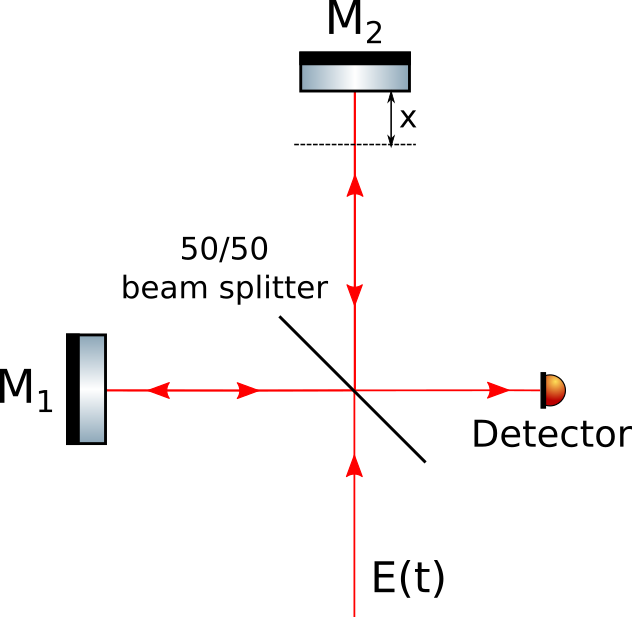
\includegraphics[width=0.55\textwidth]{Fig/Chapter1/michelson.png}
    \caption{Principle of the Michelson interferometer.}
    \label{fig:michelson}
\end{figure}


To illustrate where correlation functions come from, let us begin by taking a look at time coherence in the emblematic Michelson interferometer (see Fig.-\ref{fig:michelson}). For simplicity sake, we will not discuss spatial coherence effects and will thus consider a punctual source producing a complex light field $E(t)$ that we send into the interferometer. The intensity measured by the detector writes:

\begin{equation}
    I=\mean{\abs{E(t)+E(t-\tau)}^2}
    \label{eq:i_michelson}
\end{equation}

where $\mean{...}$ denotes the time average made by the detector and $\tau=\frac{2x}{c}$ the delay between the two interfering waves induced by the optical path difference between the two arms of the interferometer. Developing equation \ref{eq:i_michelson} we get:

\begin{equation}
    I=\mean{\abs{E(t)}^2} + \mean{\abs{E(t-\tau)}^2} + 2 {\rm{Re}} \mean{E(t) E^*(t-\tau)}
    \label{eq:def_g1}
\end{equation}

For simplicity sake, let us assume that the source is stationary to write $\mean{\abs{E(t)}^2} = \mean{\abs{E(t-\tau)}^2} = I_0$, we then obtain :

\begin{equation}
    I= 2 I_0 (1 + {\rm{Re}} (g^{(1)} (\tau))) \ , \ g^{(1)} (\tau) = \frac{ \mean{E(t) E^*(t-\tau)}}{\mean{\abs{E}^2}}
\end{equation}

We have introduced the normalized \textbf{first-order correlation function} $g^{(1)}$ that characterizes the interference term. If $E(t)$ and $E(t-\tau)$ are independent and thus uncorrelated, $\mean{E(t) E^*(t-\tau)} = \mean{E(t)} \mean{ E^*(t-\tau)}=0$ and interference cannot be observed \NOTE{corriger}. On the other hand, if there is a \textbf{correlation} between these two quantities, an interference phenomenon can be observed. 

To illustrate what kind of information are contained in this first-order correlation function, let us compute it for the simple case of a monochromatic light source of frequency $\omega_0$. The light field writes:

\begin{equation}
    E(t)=E_0 e^{i \omega_0 t}
\end{equation}

From this, we calculate the first-order correlation function:

\begin{equation}
    g^{(1)} (\tau) = \frac{|E_0|^2 \mean{e^{i\omega_0 t} e^{i \omega_0 (t-\tau)}}}{|E_0|^2} = e^{i \omega_0 \tau}
\end{equation}

The detected intensity is thus a perfect sinusoidal function of $\tau$ that is scanned by changing the position of the second mirror and thus the value of $x$:

\begin{equation}
I(x)= 2 I_0 (1+\cos(\omega_0 \frac{2x}{c}))
\end{equation}

Measuring the intensity pattern as a function of $x$ thus gives a measurement of $\omega_0$. What happens if we make things slightly more complex a light source with two monochromatic compononents $\omega_1$ and $\omega_2$? The new light field writes:

\begin{equation}
    E(t)= E_1 e^{i \omega_1 t} + E_2 e^{i \omega_2 t}
\end{equation}

Let us compute the numerator of the first-order correlation function:

\begin{equation}
       \mean{E(t) E^*(t-\tau)} & = \mean{|E_1|^2 e^{i \omega_1 \tau} + |E_2|^2 e^{i \omega_2 \tau} + E_1 E_2^* e^{i \omega_2 \tau} e^{i (\omega_1 - \omega_2)t} + E_2 E_1^* e^{i \omega_1 \tau} e^{i (\omega_2 - \omega_1)t}}  
\end{equation}

In most practical situations, the detector time average is large compared to $1/(\omega_1 - \omega_2)$, the two last terms thus get averaged out. If we consider the simple case where $|E_1|^2=|E_2|^2$, the normalized first-order correlation function writes:

\begin{equation}
    g^{(1)} (\tau) = \frac{1}{2} (e^{i \omega_1 \tau} + e^{i \omega_2 \tau})
\end{equation}

We simply get the sum of the contribution of the two frequencies. The intensity pattern as a function of $x$ is thus the sum of two cosine functions with different frequencies. Using trigonometric identities, we find that the intensity pattern consists of a "fast" oscillation of frequency $\omega_0=(\omega_1 + \omega_2)/2$, modulated by a "slow" oscillation of frequency $\Delta \omega = |\omega_1 - \omega_2|$, reducing the visibility of the interference pattern (see Fig.-\ref{fig:michelson_two_lambda}).

\begin{figure}
    \centering
    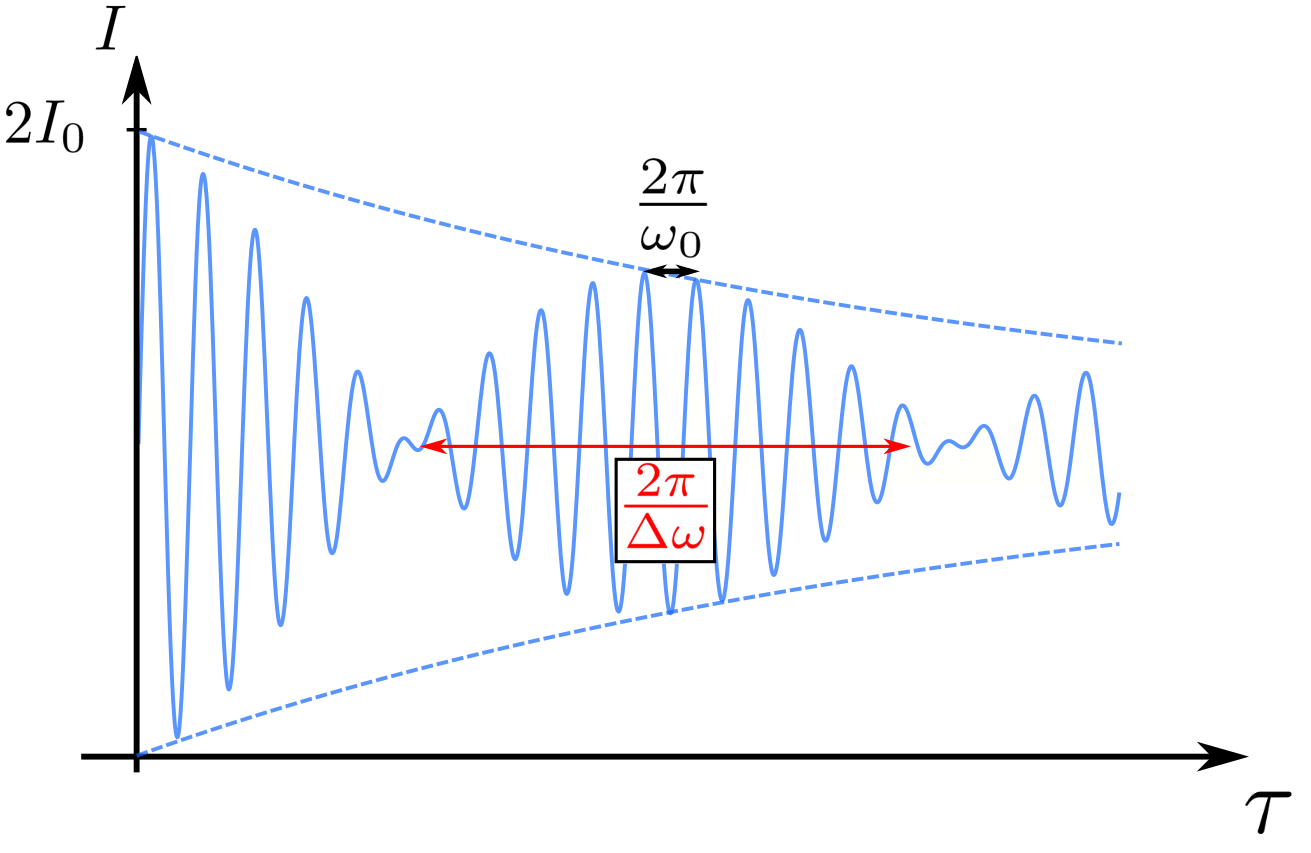
\includegraphics[width=0.78\textwidth]{Fig/Chapter1/michelson_two_lambda.png}
    \caption{Intensity pattern for a light source with two monochromatic component of frequencies $\omega_1$ and $\omega_2$. The fast oscillation of frequency $\omega_0=(\omega_1+\omega_2)/2$ is modulated by a slow oscillation of frequency $\Delta \omega = |\omega_1 - \omega_2|$.}
    \label{fig:michelson_two_lambda}
\end{figure}

Through this very simple example, we understand that the observed interference pattern strongly depends on the spectrum of the source. This is quantified by the \textbf{Wiener-Khintchine} theorem. For a source with an arbitrary spectrum $S(\omega)$, the overall intensity pattern results of the sum of the contribution of each spectral component:

\begin{equation}
    I=\int_{-\infty}^{\infty} 2 S(\omega)[1+\cos (\omega \tau)] \mathrm{d} \omega
\end{equation}

Writing $\int_{-\infty}^{\infty} S(\omega) \mathrm{d} \omega=I_{0}$ and $s(\omega)=S(\omega) / I_{0}$, we obtain

\begin{equation}
    I=2 I_{0}\left[1+\int_{-\infty}^{\infty} s(\omega) \cos (\omega \tau) \mathrm{d} \omega\right]
\end{equation}

Since $s(\omega)$ is real, we can rewrite:

\begin{equation}
    I=2 I_{0}\left[1+\mathrm{Re} \left(\int_{-\infty}^{\infty} s(\omega) \cos (\omega \tau) \mathrm{d} \omega\right)\right]
\end{equation}

From which we get, using equation \ref{eq:def_g1}:

\begin{equation}
    g^{(1)}(\tau)=\int_{-\infty}^{\infty} s(\omega) \mathrm{e}^{\mathrm{i} \omega \tau} \mathrm{d} \omega
\end{equation}

where we recognize the formula of the Fourier transform. We have thus seen that the first-order correlation function, measurable with an interferometric measurement, contains information about the spectrum of the light source. 



% Note that this is only one example in the ensemble of the many possible applications of the study of first-order correlation. We can also quote for instance the characterization of the spatial coherence of a non punctual source with the famous Young's slits experiment. 

In this introductory paragraph, we have seen a concrete and evocative example of how correlation functions can be used to obtain meaningful information about a given system, here a light source, with the simplest correlation function there is, correlating two values of the light field. At this point, the link with our initial goal, {\it i.e.} characterizing quantum many-body interacting systems, do not seem so clear. As we mentioned earlier, interactions induce correlations between several particles for which we will need higher order correlation functions. Let us now take the next step in this direction and look at \textbf{second-order correlation functions}. We will do so still in the context of optics for which this formalism was historically developed and that provides well-known, easy to understand examples.

% The same reasoning can be conducted for the spatial coherence for instance with the non less famous Young double slit experiment. 

% We will not detail here all the intricacies of the study of first-order correlation functions for different light sources. The main point to remember is that the first order correlation function is a natural way to characterize the coherence properties of a light source and thus contains a lot of meaningful information.


\subsection{Second order correlation function of light: The Hanbury Brown and Twiss effect}

The idea to use the second-correlation function of light was introduced by Hanbury Brown and Twiss in their really famous 1956 article \cite{brown1954lxxiv}, as a mean to improve the resolution of the Michelson interferometer for measuring the size of the stars. To understand how it works, we will take another approach than the one developed in the last paragraph and look at the spatial properties of the light source. 

We consider an incoherent, non-punctual, monochromatic (wavelength $\lambda$) light source and write $S$ the surface of the source. We model it as an ensemble of elementary, punctual and incoherent emitters and note their spatial location $\bm{s}$. The amplitude at a point $\bm{r}$ in an observation plane situated at distance $L$, far-away from the source so that we are in the Fraunhofer regime $L \gg \lambda, r,s$, writes:

\begin{equation}
    A(\bm{r}) \propto \int_{S} a(\bm{s}) e^{\frac{i \pi}{\lambda L}|\bm{r}-\bm{s}|^{2}} d \bm{s}
    \label{eq:amp_HBT}
\end{equation}

The second-order correlation function correlates the values of the intensity of the light field at two different points of space $\bm{r}_1$ and $\bm{r}_2$. In terms of field amplitude, it corresponds to the four-term correlator:

\begin{equation}
    G^{(2)} (\bm{r}_1,\bm{r}_2) = \mean{A^*(\bm{r}_1) A(\bm{r}_1) A^*(\bm{r}_2) A(\bm{r}_2)}
\end{equation}

All the elementary emitters are incoherent and thus each have a random phase value, determined by an uniform probability law defined on the interval $[0,2\pi]$ (\NOTE{INTRODUIRE CHAOTIC}). They thus form an ensemble of \textbf{independent} random variables with the \textbf{same statistics}. We can therefore apply the Central Limit Theorem to find that the variable $A$ follows Gaussian statistics. This allows us to simplify the four-term correlator into:

\begin{equation}
     G^{(2)} (\bm{r}_1,\bm{r}_2) = \mean{I(\bm{r}_1)} \mean{I(\bm{r}_2)} + \mean{A^*(\bm{r}_1) A(\bm{r}_2)} \mean{A(\bm{r}_1) A^*(\bm{r}_2)}
\end{equation}

We recognize in the second term the spatial counterpart of the temporal first-order correlation function discussed in the previous paragraph. Using equation \ref{eq:amp_HBT}, we obtain:

\begin{equation}
    G^{(1)}\left(\bm{r}_{1}, \bm{r}_{2}\right)=\left\langle A^*(\bm{r}_1) A(\bm{r}_2)\right\rangle \propto \iint_{S}\left\langle a^{*}(\bm{s}_1) a(\bm{s}_2)\right\rangle e^{-\frac{i \pi}{\lambda L}\left(\left|\bm{r}_{1}-\bm{s}_1\right|^{2}-\left|\bm{r}_{2}-\bm{s}_2\right|^{2}\right)} \mathrm{d} \bm{s}_1 \mathrm{d} \bm{s}_2
\end{equation}

Since the source is incoherent, we simplify $\left\langle a^{*}(\bm{s}_1) a(\bm{s}_2)\right\rangle = I(\bm{s}_1) \delta_{\bm{s}_1,\bm{s}_2}$, giving

\begin{equation}
    G^{(1)}\left(\bm{r}_{1}, \bm{r}_{2}\right) \propto \iint_{S} I(\bm{s}_1) e^{-\frac{2 i \pi}{\lambda L}\left(\bm{r}_{1}-\bm{r}_{2}\right) \bm{s}_1} \mathrm{d} \bm{s}_1 d \bm{s}_2
\end{equation}

In analogy with what we showed in the last paragraph for the temporal coherence, the first-order spatial correlation function is the Fourier transform of the spatial intensity profile. 

In a nutshell, the second-order normalized correlation function has the simple expression:

\begin{equation}
    \gtwo (\bm{r}_1,\bm{r}_2) = \frac{\mean{I(\bm{r}_1)} \mean{I(\bm{r}_2)} + \mean{A^*(\bm{r}_1) A(\bm{r}_2)} \mean{A(\bm{r}_1) A^*(\bm{r}_2)}}{\mean{I(\bm{r}_1)}\mean{I(\bm{r}_2)}} = 1 + |g^{(1)}(\bm{r}_1,\bm{r}_2)|^2
\end{equation}

Inter


\subsection{HBT with the perfect Bose gas}

\section{Bogoliubov theory of the weakly-interacting gas}

Thus far, we have familiarized ourselves with correlation functions and seen through a few examples the kind of information they contain. We will now try to use this tool to study a many-body problem, the weakly-interacting homogeneous Bose gas, {\it i.e.} an ensemble of bosonic particles with weak contact interactions in a box of volume $V$. The theoretical description of this system has been developed by Nikolay Bogoliubov in his famous 1947 article \cite{bogoliubov1947}. In this section, we will remind the main lines of Bogoliubov's approach and see what it tells us in terms of correlation functions.

\subsection{Bogoliubov approximation}

\NOTE{Etapes avant?}

The Hamiltonian of the weakly-interacting Bose gas with contact interactions writes:

\begin{equation}
    \hat{H}=\sum_{\bm{k}}\frac{\hbar^2 k^2}{2m} \hat{a}^{\dagger}_{\bm{k}}  \hat{a}_{\bm{k}} +  \frac{g}{2V} \sum \hat{a}^{\dagger}_{\bm{k_1}+\bm{k_3}} \hat{a}^{\dagger}_{\bm{k_2}-\bm{k_3}} \hat{a}_{\bm{k_1}} \hat{a}_{\bm{k_2}} 
\end{equation}

\noindent where $g=\dfrac{4 \pi \hbar^2 a_s}{m}$ is the strength of the interactions with $a_s$ the s-wave sacttering length. \NOTE{DILUTENESS?} In order to simplify this Hamiltonian, we use the Bogoliubov approximation that relies on two points:

\begin{itemize}
    \item Since the interactions are weak, we assume that the number of atoms outside of the BEC is small. We therefore only consider interaction processes removing two particles from the BEC or bringing back two particles into the BEC. Mathematically speaking, we drop all terms higher than quadratic in $\hat{a}_{\bm{k}}$ and $\hat{a}^{\dagger}_{\bm{k}}$.
    \item The number of atoms $\NBEC$ is assumed to be very large. Therefore, we replace $\hat{a}_{\bm{0}}$ and $\hat{a}^{\dagger}_{\bm{0}}$ by $\sqrt{\NBEC}$. 
\end{itemize}

With these approximation, the simplified Hamiltonian writes:

\begin{equation}
    H_{\rm{bogo}}=\sum_{\bm{k}}\frac{\hbar^2 k^2}{2m} a^{\dagger}_{\bm{k}}  a_{\bm{k}} +  \frac{gn}{2} \sum_{\bm{k}} (a^{\dagger}_{\bm{k}} a^{\dagger}_{-\bm{k}} +a_{\bm{k}} a_{-\bm{k}})+\frac{gn\NBEC}{2}
\end{equation}

What we now want to is diagonalize the Hamiltonian. This is achieved through the linear Bogoliubov transformation where we introduce a new operator:

\begin{equation}
    \hat{b}_{\bm{k}}=u_{\bm{k}} \hat{a}_{\bm{k}} + v_{-\bm{k}} \hat{a}^{\dagger}_{-\bm{k}}
\end{equation}

To determine the expression of the coefficients $u_{\bm{k}}$ and $v_{\bm{k}}$, we impose that the new operator $\hat{b}_{\bm{k}}$ follows the bosonic operator commutation rule:

\begin{equation}
    [\hat{b}_{\bm{k}},\hat{b}^{\dagger}_{\bm{k}'}]= \delta_{\bm{k},\bm{k}'}
\end{equation}

This gives $u_{\bm{k}}^2 -  v_{-\bm{k}}^2 =1$. We can therefore write $u_{\bm{k}}={\rm cosh}(\alpha_{\bm{k}})$ and $v_{-\bm{k}}={\rm sinh}(\alpha_{\bm{k}})$ and look to determine $\alpha_{\bm{k}}$. This value must be chosen so that the coefficients of the terms in $\hat{b}^{\dagger}_{\bm{k}} \hat{b}^{\dagger}_{-\bm{k}}$ and $\hat{b}_{\bm{k}} \hat{b}_{-\bm{k}}$ vanish. We obtain an additional equation:

\begin{equation}
    \frac{g n}{2}\left(u_{\bm{k}}^{2}+v_{-\bm{k}}^{2}\right)+\left(\frac{k^{2}}{2 m}+g n\right) u_{\bm{k}} v_{-\bm{k}}=0
\end{equation}

from which we finally obtain after a few calculations using the properties of hyperbolic functions:

\begin{equation}
    u_{\bm{k}}, v_{-\bm{k}}=\pm\left(\frac{\hbar^2k^{2} / 2 m+g n}{2 \varepsilon(k)} \pm \frac{1}{2}\right)^{1 / 2}
\end{equation}

with 

\begin{equation}
    \varepsilon(k)=\sqrt{\frac{\hbar^2 k^2}{2m}(\frac{\hbar^2 k^2}{2m}+2gn)}
\end{equation}

the famous Bogoliubov dispersion relation. The Hamiltonian has now been diagonalized and writes:

\begin{equation}
    \hat{H}_B = \sum_{\bm{k}}\varepsilon(k) b^{\dagger}_{\bm{k}}  b_{\bm{k}}+E_0
\end{equation}

The system of interacting particles has thus been transformed into a system of non-interacting Bogoliubov quasi-particles associated to creation and annihilation operators $\hat{b}^{\dagger}_{\bm{k}}$ and $\hat{b}_{\bm{k}}$ with a dispersion relation $\varepsilon(k)$. The prediction of this excitation spectrum is one of the key results of Bogoliubov theory that we will now discuss in further details.

\subsection{Spectrum of excitations}
\label{sec:spectrum}

The Bogoliubov dispersion relation has two clear asymptotic trends for small and high momentum values. For low values of $k$, using $\frac{\hbar^2 k^2}{2m} \ll 2gn$, we obtain:

\begin{equation}
    \varepsilon(k) \underrel{k \to 0}{=} \hbar k \sqrt{\frac{gn}{m}}
\end{equation}

The dispersion relation takes a phonon-like linear dispersion form where the sound velocity is $c=\sqrt{\dfrac{gn}{m}}$. In this regime, the Bogoliubov quasi-particles are thus phonons that can be sen as a coherent superposition of a forward and backward propagating real particles $\hat{b}_{\bm{k}}=u_{\bm{k}} \hat{a}_{\bm{k}} + v_{-\bm{k}} \hat{a}^{\dagger}_{-\bm{k}}$ with $\abs{u_{\bm{k}}} \simeq \abs{v_{-\bm{k}}}$.

On the other hand, at high values of $k$, the dispersion relation becomes the one of free particles:

\begin{equation}
    \varepsilon(k) \underrel{k \to +\infty}{=} \frac{\hbar^2 k^2}{2m}
\end{equation}

In terms of operators, $v_k \underrel[c]{k \to +\infty}{=} 0$ and $u_k \underrel[c]{k \to +\infty}{=} 1$ so $\hat{b}_{\bm{k}}\underrel[c]{k \to +\infty}{=}\hat{a}_{\bm{k}}$, a quasi-particle is equivalent to a real particle. 

The transition between the two regimes occurs when $\frac{\hbar^2 k^2}{2m} \simeq gn$, it thus convenient to define a characteristic length associated to this momentum range:

\begin{equation}
    \xi = \sqrt{\frac{\hbar^2}{2mgn}}
\end{equation}

This length is called the \textbf{healing length} \NOTE{COMPLETER?}. We will use it later when discussing our experimental results to characterize the region of the Bogoliubov spectrum we are probing.

The Bogoliubov spectrum of excitation has been a very successful theoretical prediction observed experimentally in a large variety of systems \cite{miller1962, steinhauer2002excitation, ozeri2005, fontaine2018, stepanov2019}. However, the Bogoliubov theory also gives an additional prediction for the \textbf{ground-state} of the system.

\begin{figure}
    \centering
    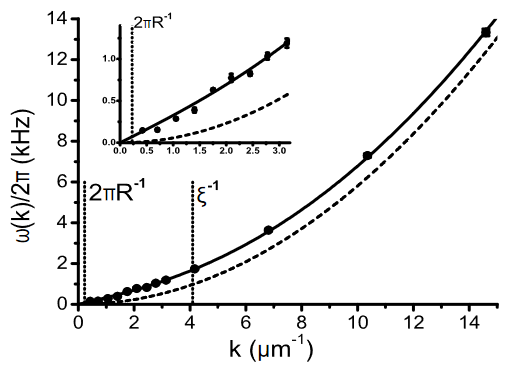
\includegraphics[width=0.65\textwidth]{Fig/Chapter1/bogo_steinhauer.png}
    \caption{Experimental observation of the Bogoliubov excitation spectrum (Steinhauer {\it et al.} \cite{steinhauer2002excitation}). The phononic and free particle parts are clearly identifiable. The inset shows a zoom on the linear part of the spectrum and the dashed the free particle spectrum. $\xi$ is the healing length of the condensate.}
    \label{fig:my_label}
\end{figure}

\subsection{The quantum depletion}

As we have just seen, the Bogoliubov approach describes the weakly-interacting Bose gas excitations as non-interacting quasi-particles. They therefore behave as ideal bosons and follow the Bose distribution:

\begin{equation}
    \langle b^{\dagger}_{\bm{k}}  b_{\bm{k}} \rangle=\frac{1}{e^{-\varepsilon(k)/(k_B T)}-1} 
    \label{eq:bose_qp}
\end{equation}

Naturally, at $T=0$, the population of quasi-particles is null: $\langle b^{\dagger}_{\bm{k}}  b_{\bm{k}} \rangle_{T=0}=0$. That being said, let us now write the population of real particles for a given momentum $k \neq 0$:

\begin{equation}
    \langle a^{\dagger}_{\bm{k}}  a_{\bm{k}} \rangle=\textcolor{blue}{(|u_k|^2+|v_k|^2)\langle b^{\dagger}_{\bm{k}}  b_{\bm{k}} \rangle} + \textcolor{green}{|v_k|^2}
\end{equation}

The blue term corresponds to the Bogoliubov excitations populated by temperature. We will call the fraction of particles removed from the condensate this way the \textcolor{blue}{\textbf{thermal depletion}}. This fraction vanishes at $T=0$. Very interestingly, we see the apparition of an additional term \textcolor{green}{$|v_k|^2$} that results from the non commutation of the bosonic creation and annihilation operators, the signature of an essentially quantum phenomenon. This term tells us that $\langle a^{\dagger}_{\bm{k}}  a_{\bm{k}} \rangle_{T=0} \neq 0$, meaning that there are some atoms outside of the BEC with a non zero momentum in the ground state! Under the interplay between interactions and quantum fluctuations, some atoms are removed from the BEC and obtain a non zero momentum. The fraction of these atoms is called the \textcolor{green}{\textbf{quantum depletion}}. 

We are thus looking at a system which seems to fall into our general area of interest described in the introduction of this thesis, namely many-body systems with interactions displaying quantum behaviors. The weakly-interacting Bose gas shows the advantage to be one of the conceptually simplest many-body systems for which a theory can be derived as we just have shown. As explained in the beginning of this chapter, many-body systems are often efficiently characterized by correlation functions. Let us now discuss what are the relevant correlation functions to study for the weakly-interacting Bose gas.


\section{Two-body correlations in the weakly-interacting Bose gas}

\subsection{k/-k correlations in the many-body ground state}

Let us now come back to the ground-state of the weakly-interacting Bose gas and the quantum depletion. We will now try to build a microscopic, physically meaningful picture of how the quantum depletion emerges. We remind that a key ingredient of the Bogoliubov theory is that the only considered interaction processes are the ones involving two particles of the BEC or two particles outside of the BEC being brought into it. From this consideration, we understand that the atoms belonging to the quantum depletion were initially in the BEC and were removed from it after undergoing a two-body interaction process. The interaction process populating the quantum depletion thus involves two atoms in the BEC with a momentum $k \simeq 0$. To conserve the overall momentum, the two atoms leaving the BEC then have opposite momenta $\bm{k}$ and $-\bm{k}$ and form a momentum correlated pair. This falls exactly into the kind of signal we are interested in, namely correlations between several particles, here two, caused by a quantum, interaction-induced effect.

The common factor with quantum effects is that they usually defy our intuition built on our observation of the everyday world, well described by classical physics. In this case, the "quantum weirdness" comes from the fact this process seems to violate the conservation of energy: the two at atoms initially at rest each have an extra kinetic energy $\frac{\hbar^2 k^2}{2m}$ after the interaction process giving them the $\bm{k}$ and $-\bm{k}$ momenta. Naturally, the conservation of energy is still well respected here. The apparent contradiction comes from the fact that it is conceptually wrong to isolate two atoms in the BEC. The ground-state must rather be understood as a single many-body wave-function describing indistinguishable atoms, with a non zero component for momentum values $k \neq 0$. The energy of the many-body ground state of the weakly-interacting Bose gas contains a small correction that corresponds to the presence of the \kmk pairs of the quantum depletion. This small correction is called the Lee-Huang-Yang correction, named after the authors of the seminal 1957 article \cite{lee1957} that first predicted the presence of the \kmk pairs.

\subsection{Finite temperature effects} functions to detect them as we will now discuss.



\subsection{Second order correlation functions within Bogoliubov theory}

We start by describing the general case of the two-body correlator between two modes $\bm{k}$ and $\bm{k'}$:

\begin{equation}
    G(\bm{k},\bm{k}')=\langle \hat{a}^{\dagger}({\bm k}) \hat{a}^{\dagger}({\bm k}') \hat{a}({\bm k}) a({\bm k}') \rangle
\end{equation}

As we have seen in the previous section, the Bogoliubov Hamiltonian is diagonal in the quasi-particle basis. All quantum thus have Gaussian statistics, allowing us to use Wick's theorem to simplify correlator:

\begin{equation}
    G(\bm{k},\bm{k}')=\langle \hat{a}^{\dagger}({\bm k}) \hat{a}^{\dagger}({\bm k}') \rangle \mean{\hat{a}({\bm k}) a({\bm k}')} + \langle \hat{a}^{\dagger}({\bm k}) \hat{a}({\bm k}) \rangle \langle \hat{a}^{\dagger}({\bm k}') a({\bm k}') \rangle + \langle \hat{a}^{\dagger}({\bm k}) \hat{a}({\bm k}') \rangle \langle \hat{a}^{\dagger}({\bm k}') a({\bm k}) \rangle
\end{equation}

We end up with three different terms:

\begin{itemize}
    \item The first term equals $| \langle \hat{a}^{\dagger}({\bm k}) \hat{a}^{\dagger}({\bm k}') \rangle |^2$ and is non zero only when $\bm{k}'=-\bm{k}$. This corresponds to the \kmk correlations.
    \item We recognize in the second term the product of the first-order correlation functions for modes $\bm{k}$ and $\bm{k}'$ which is simply the product of the momentum densities $\rho(\bm{k}) \rho(\bm{k}')$.
    \item The third term equals $| \langle \hat{a}^{\dagger}({\bm k}) \hat{a}({\bm k}') \rangle |^2$ and is non zero only when $\bm{k}'=\bm{k}$. This correspond to the Hanbury Brown and Twiss effect or bosonic bunching described earlier.
\end{itemize}

We regroup the two last terms in the function $G^{(2)}_{N}({\bm k},{\bm k}')= \rho({\bm k})\rho({\bm k}') + | \langle \hat{a}^{\dagger}({\bm k}) \hat{a}({\bm k}') \rangle |^2$ that we call the \textbf{normal} correlation function as the operators are normally ordered to match the interpretation of the detection of two particles \NOTE{FISHY}. In opposition, we introduce for the last term the function $G^{(2)}_{A}({\bm k},{\bm k}')=| \langle \hat{a}^{\dagger}({\bm k}) \hat{a}^{\dagger}({\bm k}') \rangle |^2 $ that we call the \textbf{anomalous} correlation function. 

We end up with two correlation functions of interest well separated in momentum space and containing very different types of information. On the one hand, the normal correlations correspond to close-by correlations and bosonic bunching: this effect is caused by chaotic statistics and this correlation function thus gives information about the statistics of the system. On the other hand, the anomalous correlations correspond to \kmk correlations and reveal the quantum coherences of the many-body ground state.

\NOTE{VOIR CETTE TRANSITION} While our main goal will be to measure the anomalous \kmk correlations for the reasons mentioned earlier, it will also be of great interest to measure the local normal correlations as a point of comparison. 


% As we will see in Chapter 4, the clear separation of the contribution of the two correlation functions in momentum space (close-by or \kmk) allows to measure them separately on the same experimental data set.



Now that we have formed a clear picture of the kind of correlation functions we want to measure, we need to identify the key experimental ingredients necessary to observe such signals. The principal one is to have an experiment capable of measuring the momentum of individual atoms in momentum space and not only the momentum density as in most cold atoms experiment. This will be the subject of Chapter 3. 

In addition, there are several key features of the \kmk correlation signal that we need to properly understand to design an experimental scheme where the \kmk correlation signal can be properly detected.


\subsection{Momentum extent of the quantum depletion}

A crucial aspect of studying the correlations in the depletion is the ability to separate the depleted atoms from the condensed ones. As a matter of fact, the BEC is a fully coherent state with macroscopic occupation of a single mode. In analogy with laser light in optics, the statistics of the BEC are not chaotic and no bosonic bunching can therefore be observed. In addition, no \kmk correlations are expected for atoms belonging to the condensate. Furthermore, the number of condensed atoms is very often way larger than the number of depleted atoms. This has a direct consequence for our measurement: if we are unable to remove condensed atoms from the analysis, they will entirely drown out the correlation signals of the depletion.

Fortunately, the BEC and the depletion extent in momentum space are very different. Positions and momenta are related to one other by means of Fourier transform. This tells us that the typical momentum width of the condensate is $1/L_{\rm{BEC}}$ where $L_{\rm{BEC}$ is the spatial size of the BEC. On the other hand, the typical momentum width of the quantum depletion is $1/\xi$. \NOTE{WHAT ABT THERMAL DEPLETION?}. Since $\xi \ll L_{\rm{BEC}}$, $1/\xi \gg 1/L_{\rm{BEC}}$ meaning that the depletion extends on a much larger momentum area than the BEC. This provides us with a natural to separate the condensate from its depletion and defines one of the experimental ingredient: we need an experimental setup allowing us to exclude \NOTE{FINIR MOCHE}


\subsection{Finite temperature effects}

Another parameter that we must be very careful of is the temperature. In an ideal situation, we would conduct the experiment at zero temperature where the depletion is entirely quantum and all atoms consequently \kmk paired. Obviously this is impossible to do in practice and the experiment will always be done at finite temperature.

Temperature is an absolutely crucial parameter when measuring \kmk correlations as it sets the population of the thermal depletion, {\it i.e.} the population of the Bogoliubov quasi-particles (see equation \ref{eq:bose_qp}). At first glance, if the temperature is too high, the thermally depleted atoms will significantly outnumber the quantum depleted ones and it will then be impossible to detect the \kmk correlations. However, this observation needs to be nuanced as the thermal depletion can also show \kmk correlations, albeit for different reasons than the quantum depletion. As discussed in \ref{sec:spectrum}, for low $k$ values such as $k \xi \ll 1$, the Bogoliubov quasi-particles have a strong phononic character and therefore exhibits \kmk correlations in terms of real particles. Nonetheless, this low $k$ region corresponds more or less to the region that will need to be removed to exclude the BEC from the analysis (experimental numbers will be given in Chapter 4). We therefore do not have to care for the contribution of the thermal depletion to the \kmk correlation signal that will in our case only reflect the quantum depletion correlations.

In order to quantify the effect of temperature, we compare the typical thermal energy $k_B T$ to the chemical potential of the condensate $\mu$ quantifying the effect of interactions. We aim to be in an experimental regime where $k_B T \ll \mu$, {\it i.e.} where interactions effects dominate temperature effect. The first idea that comes to mind is then to reduce the temperature as much as possible. We however quickly hit a brick wall: the lowest temperature in ultracold experiments are obtained through evaporative cooling. This process will detailed in Chapter 3 but we can quickly give here the main idea, which is to remove the hottest atoms of the gas to let the other thermalize at a colder temperature. We quickly see the problem here: if we further evaporatively cool the gas, we lose more atoms, reduce the density therefore reduce the effect of interactions and make no progress. This method allows us to typically reach $k_B T \sim \mu$ which is not sufficient to ensure the proper detection of \kmk correlations.

We are thus left with one only possible solution which is to increase the interactions. To this end, we will use a \textbf{3D optical lattice}. As a brief overview, a 3D optical lattice is formed by interference of 3 pairs of countra-propagating beams, one for each direction of space. The interferences create a sinusoidal potential trapping the atoms at the minimum (\NOTE{CHECK}) of the light intensity profile, {\it i.e.} in periodically arranged wells, mimicking a condensed matter crystal. In our case, the density will increased inside of the individual wells as a result of higher local trapping frequencies, allowing us to increase the strength of interactions.

\section{Conclusion}

In this chapter, we have shown that correlation functions are an important and powerful tool that was first developed to describe classical effects of the light such as interferences. \NOTE{BLAH BLAH HBT}. These functions were then latter used in atomic physics and are of great interest to characterize \textbf{many-body interacting} systems. We made the proposition to study one of the simplest many-body system, the weakly-interacting Bose gas described by the Bogoliubov theory that we detailed the main lines of. We have shown that the Bogoliubov theory predicts the existence of the quantum depletion, a fraction of atoms removed from the condensate through the interplay between interactions and quantum fluctuations, and that we expect these atoms to form \kmk correlated pairs, that we will aim to detect by measuring second-order correlation functions. To this end, we have devised that our experimental setup should:

\begin{itemize}
    \item Detect single atoms in momentum space.
    \item Isolate the contribution of the depletion from the one of condensed atoms.
    \item Be in the low-temperature regime where interactions dominate temperature effects $k_B T \ll \mu $. 
\end{itemize}

We decided for this last point to use 3D optical lattices that we will discuss in details in the next chapter of this thesis.